\documentclass[a4paper]{report}

\usepackage[utf8]{inputenc}
\usepackage[T1]{fontenc}
\usepackage{textcomp}
\usepackage{amsmath, amssymb}
%\usepackage{amsthm}
\usepackage{xcolor}
\usepackage{tcolorbox}
\tcbuselibrary{theorems}
\newtcbtheorem
  []% init options
  {definition}% name
  {Definition}% title
  {%
    colback=green!5,
    colframe=green!35!black,
    fonttitle=\bfseries,
  }% options
  {def}% prefix

\newtcbtheorem
  []% init options
  {theorem}% name
  {Theorem}% title
  {%
    colback=red!5,
    colframe=red!35!black,
    fonttitle=\bfseries,
  }% options
  {thrm}% prefix

\newtcbtheorem
  []% init options
  {example}% name
  {Example}% title
  {%
    colback=blue!5,
    colframe=blue!35!black,
    fonttitle=\bfseries,
  }% options
  {expl}% prefix

\title{Discrete Math Notes}
\author{Allen Li}
% figure support
\usepackage{graphicx}
\graphicspath{ {./images/} }
\usepackage{import}
\usepackage{xifthen}
\pdfminorversion=7
\usepackage{pdfpages}
\usepackage{transparent}
\newcommand{\incfig}[1]{%
    \def\svgwidth{\columnwidth}
    \import{./figures/}{#1.pdf_tex}
}
\DeclareMathSymbol{\lsim}{\mathord}{symbols}{"18}
\usepackage{hyperref}
\hypersetup{
    colorlinks,
    citecolor=black,
    filecolor=black,
    linkcolor=black,
    urlcolor=black
}

\begin{document}
\maketitle

\newpage
\tableofcontents{}
\newpage

\chapter{Speaking Mathematically}

\section{Statements}

\subsection{The Three Types of Statements}

\begin{enumerate}
    \item Universal Statement: Statement that applies "for all"
        \begin{itemize}
            \item Ex: For all real numbers $x$, $x^2 \ge 0$
            \item Key Words: "For All"
        \end{itemize}
    \item Conditional Statement: If one thing is true then some other thing must be true
        \begin{itemize}
            \item Key Words: "If, then"
        \end{itemize}
    \item Existential Statement: Statement that says there is at least one thing for which property is true
        \begin{itemize}
            \item There exists an even prime number.
            \item Key Words: "There exists"
        \end{itemize}
    We use these three statements in order to classify different statements.
    
\end{enumerate}

\subsection{Universal Conditional Statements}

Ex: For all real numbers, if $|x| > 1$, then  $x^2 > 1$.

This statement is universal because it has the "for all", and conditional because it has "if".

\subsection{Universal Existential Statement}

Ex: For all integers $n$, there exists another integer $m$, such that $n < m$.

This statement is universal again because it has the "for all", and existential because of the "there exists".

\subsection{Existential Universal Statement}

Ex. There exists a positive integer that is less than all the positive integers.

See above reasoning.

\section{Set Builder Notation}

A set is simply defined as a collection of objects. The size of a set is the number of unique elements in the set.

\subsection{Set Roster Notation}

\begin{itemize}
    \item Example set: $A = \{a, b, c\}$
    \item As shown, sets can include anything.
\end{itemize}

\subsection{Set Builder Notation}

\begin{itemize}
    \item Example set: $A = \{ x \in \mathbb{R} \mid -1 \le  x < 5 \}$
    \item $0 \in A$, $-2 \not\in A$
    \item Empty Set: $\{\}, \phi$
    \item Universal Set: $u$, set containing all objects, all other sets are proper subsets.
    \item Subsets:  $A \subseteq B$ if for any element $a \in A$, $a \in B$
    \item By definition, $\phi \subseteq A$
    \item Proper subset: $A \subset B$ means all elements in A are also in B, and there exist elements in B that do not exist in A.
    \item $\forall $: for all, $\exists $: there exists
\end{itemize}

We actually cannot use set roster notation most of the time. It is not countable.

\subsection{Cartesian Products}

\begin{itemize}
    \item $A \times B = \{(x, y)  \mid x \in A, y \in B\}$
    \item Number of elements in $A \times B$ = sizes multiplied together
    \item This was introduced in an effort to introduce ordered pairs (differentiation of $(a, b)$ and $(b, a)$ )
    \item Because of this, $A \times B \neq B \times A$
\end{itemize}

\section{The Language of Relations and Functions}

\begin{enumerate}
    \item Relations on sets
        \begin{itemize}
            \item Definition: a relation from set $A$ to set $B$ is a subset of $A \times B$. More formally, for some relation $x$, $x \subseteq A \times B$
            \item We denote a relation between $x_1$ and $x_2$ as $x_1 \: R \: x_2$ provided that $x$ is in  $A \times B$.
            \item It can be proved intuitively that a set with $n$ elements has  $2^n$ subsets.
            \item Domain and co domain of $A \times B$ is simply $A$ and  $B$ respectively.
        \end{itemize}
    \item Function from A to B
        \begin{itemize}
            \item Definition: a function is a relation such that $\forall x \in A, \exists y \in B  \mid (x, y) \in F$ where $F: A \mapsto B$
            \item If $(x, y) \in F$ and $(x, z) \in F$ then $(y, z) \in F$.
            \item In other words, every element in $A$ must have exactly one distinct image.
        \end{itemize}
    \item Extra Function Terminology
        \begin{itemize}
            \item Squaring function: $x \mapsto x^2$
            \item Successor function: $x \mapsto x + 1$
            \item Constant function: $x \mapsto C$
        \end{itemize}
\end{enumerate}

\chapter{The Logic of Compound Statements}

\section{Logical Form and Logical Equivalence}

An argument is a sequence of statements aimed at demonstrating the truth of an assertion.

\begin{itemize}
    \item The assertion at the end of the sequence is called the conclusion, and the preceding statements are called premises.
    \item We commonly use the variables $p$ $q$ and $r$ to represent component sentences.
\end{itemize}

A statement (or proposition) is a sentence that is true or false but not both.

Further terminology:

\begin{itemize}
    \item The symbol $\lsim$ denotes not, $\land$ denotes and, and  $\lor$ denotes or.
    \item And, or, and not can easily be represented using truth tables.
    \item Set up the truth table such that each group of columns builds off of the last.
    \item Two statement forms are logically equivalent iff they have identical truth table outputs. This is represented as $P \equiv Q$.
    \item Tautology \textbf{t}: A statement form that is always true regardless of the truth values substituted
    \item Contradiction \textbf{c}: opposite of tautology
    \item $p \land \textbf{t} \equiv p$,  $p \lor \textbf{c} \equiv p$.
    \item Absorption laws: $p \lor (p \land q) \equiv p$, $p \land (p \lor q) \equiv p$
    \item See page 35 of the Discrete Math Textbook for a complete table on logical equivalences.
\end{itemize}

De Morgan's Laws: $\lsim(p \land q) \equiv \lsim p \lor \lsim q$,  $\lsim (p \lor q) \equiv \lsim p \land \lsim q$.

Caution: De Morgan's Laws can only be used between complete statements on each side.

\section{Conditional Statements}

Logic flows from a hypothesis to a conclusion. The aim is to frame it as an "if, then". Given hypothesis $p$ and conclusion $q$, we represent this as \[
p \rightarrow q
.\] 

The only combination of circumstances in which you would call a conditional sentence false occurs when the hypothesis is true and the conclusion is false. If the statement is true because the hypothesis is false, this is called vacuously true.

Note that in order of operations, $\to $ is performed last, and also note that \[
p \to q \equiv p \lor \lsim q
.\].

Helpful Information:
\begin{itemize}
    \item The negation of "if p then q" is logically equivalent to "p and not q".
    \item $p \to q \equiv \lsim q \to \lsim p$.
    \item While the converse is not equivalent to the statement, the converse is logically equivalent to the inverse.
    \item $p$ \textbf{only if} $q$ means "if $p$ then $q$".
    \item Biconditional: "if and only if" is true if both statements have the same value.
\end{itemize}

\subsection{Necessary and Sufficient Conditions}

\begin{itemize}
    \item $r$ is a sufficient condition for $s$ means "if $r$ then $s$"
    \item $r$ is a necessary condition for $s$ means "if not $r$ then not $s$"
\end{itemize}

\section{Valid and Invalid Arguments}

\subsection{Arguments Terminology}

\begin{itemize}
    \item \textbf{Argument}: sequence of statements
    \item All statements in an argument except for the final one are called premises
    \item The final statement is called a conclusion.
    \item An argument form being valid means that if the resulting premises are all true, the conclusion is true.
    \item \textbf{Critical row}: role of the truth table in which all premises are true. If the conclusion in every critical row is true, the argument form is valid.
    \item \textbf{Syllogism}: argument form consisting of two premises and a conclusion. The first and second premises in a syllogism are the major and minor premises respectively.
    \item \textbf{Modus ponens}: If $p$ then $q$. $p$. $\therefore q$. Modus ponens means "method of affirming" in Latin.
    \item \textbf{Modus tollens}: If $p$ then $q$. $\lsim q, \therefore \lsim p$. Modus tollens means "method of denying" in Latin.

\end{itemize}

\subsection{Rule of Inference}

Rule of Inference: form of argument that is valid. Below are some helpful Rules of Inference.
\begin{itemize}
    \item \textbf{Generalization}: $p \therefore p \lor q$
    \item \textbf{Specialization}: $p \land q \therefore p$
    \item \textbf{Elimination}: $p \lor q, \lsim q \therefore p$
    \item \textbf{Transitivity}: $p \to q, q \to r \therefore p \to r$
    \item \textbf{Proof by casework}: $p \lor q, p \to r, q \to r \therefore r$
\end{itemize}

\subsection{Fallacies}

\begin{itemize}
    \item Using ambiguous premises
    \item Assuming that is to be proved
    \item Jumping to a conclusion
    \item Assuming the converse to be true.
    \item Assuming the inverse to be true.
    \item An argument is sound if and only if it is valid and all its premises are true.
\end{itemize}

\subsection{Contradiction Rule}

$\lsim p \to c \therefore p$, in other words, if you can prove that an assumption leads to a contradiction, then you have proved that the assumption is false.

\chapter{The Logic of Quantified Statements}

\section{Predicates and Quantified Statements I}

\subsection{Terminology}

\begin{itemize}
    \item \textbf{Predicate Calculus}: Symbolic analysis of predicates and quantified statements
    \item \textbf{Statement Calculus}: Symbolic analysis of ordinary compound statements (see Sections 2.1-2.3)
    \item \textbf{Predicate}: part of the sentence from which the subject has been removed. A predicate is a predicate symbol together with predicate variables. 
        Predicates become statements when specific values are substituted for the variables.
        \begin{itemize}
            \item Note that predicates can be obtained by removing some or all the nouns from a statement.
        \end{itemize}
    \item \textbf{Predicate symbols}: variables to stand for predicates that act as functions that take in predicate variables
    \item \textbf{Domain of a predicate variable}: set of all values that may be substituted in place of the variable.
    \item \textbf{Truth set of $P(x)$}: set of all elements of $D$ that make $P(x)$ true when they are substituted for $x$.
        \[
            \{x \in D  \mid P(x)\}
        .\] 
\end{itemize}

\subsection{The Universal Quantifier: $\forall $}

\begin{definition}{Universal Statement}{label}
    Let $Q(x)$ be a predicate and $D$ the domain of $x$. A \textbf{universal statement} (statement
    of the form $\forall x \in D, Q(x)$) is true if, and only if, $Q(x)$ is true for every $x$ in $D$. 
    It is false if there is a counterexample.
\end{definition}
One way to show that a universal statement is true is by showing that there are no counterexamples.
This is called the \textbf{method of exhaustion}.

\subsection{The Existential Quantifier: $\exists $}

\begin{definition}{Existential Statement}{label}
    Let $Q(x)$ be a predicate and $D$ the domain of $x$. An \textbf{existential statement} (statement
    of the form $\exists x \in D, Q(x)$) is true if, and only if, $Q(x)$ is true for at least one $x$ in $D$. 
    It is false if and only if $Q(x)$ is false for all $x$ in $D$.
\end{definition}

\subsection{Equivalent Forms of Universal and Existential Statements}

Observe that ($\forall x \in U$, if $P(x)$ then $Q(x)$) can always be rewritten as
$\forall x \in D, Q(x)$ by narrowing $U$ to be the domain $D$ where  $D$ consists of all values
$x$ that make $P(x)$ true.

\subsection{Implicit Quantification}

\begin{definition}{Implication Notation}{label}
    Let $P(x)$ and $Q(x)$ be predicates.
    \begin{itemize}
        \item $P(x) \implies Q(x) \equiv \forall x, P(x) \to Q(x)$, meaning every element in the truth
            set of $P(x)$ is also in the truth set of $Q(x)$.
        \item $P(x) \Leftrightarrow Q(x) \equiv \forall x, P(x) \leftrightarrow Q(x)$, meaning the two
            predicates have identical truth sets.
    \end{itemize}
\end{definition}

\section{Predicates and Quantified Statements II}

This section contains rules for negating quantified statements and additional extensions to quantified statements.

\begin{theorem}{Negation of a Universal Statement}{label}
    \[
    \lsim (\forall x \in D, Q(x)) \equiv \exists x \in D  \mid \lsim Q(x)
    .\] 
    In other words, the negation of a universal statement is that there exists a counterexample.
\end{theorem}

\begin{theorem}{Negation of an Existential Statement}{label}
    \[
        \lsim (\exists x \in D  \mid Q(x)) \equiv \forall x \in D, \lsim Q(x)
    .\] 
    In other words, the negation of an existential statement is the universal statement "none are" or "all are not".
\end{theorem}

Note that using the Negation of a Universal Statement theorem, we can find the negation of a universal conditional statement by
negating the quantifier and the conditional "separately".

\[
    \lsim (\forall x, P(x) \to Q(x)) \equiv \exists x  \mid P(x) \land ~Q(x)
.\] 

\subsection{Relation among $\forall ,\exists ,\land, \lor$}

Note that \[
    \forall x \in D, Q(x) \equiv Q(x_1) \land Q(x_2) \land \ldots \land Q(x_n)
.\] 
Similarly, \[
    \exists x \in D  \mid Q(x) \equiv Q(x_1) \lor Q(x_2) \lor \ldots \lor Q(x_n)
.\] 
Using this, we can easily prove the above two theorems using DeMorgan's Laws.
Additionally, note that contrapositives, converses, and inverses extend to universal conditional statements as well, and there is no need
to flip the quantifier when finding these.

\subsection{Necessary and Sufficient Conditions}

\begin{definition}{Sufficient/Necessary Conditions}{label}
    \begin{itemize}
        \item "$\forall x, r(x)$ is a \textbf{sufficient condition} for $s(x)$" means "$\forall x, r(x) \to s(x)$".
        \item "$\forall x, r(x)$ is a \textbf{necessary condition} for $s(x)$" means "$\forall x, \lsim r(x) \to \lsim s(x)$".
    \end{itemize}
\end{definition}

\section{Statements with Multiple Quantifiers}

When there are multiple quantifiers, we perform the quantifiers in the order that they are stated. In terms of coding, it may be helpful to think
of the first quantifier as the outer loop and the second quantifier as the inner loop in a case with 2 quantifiers.
Amazingly, note that the order of the quantifiers only matters between $\forall $ and $\exists $.

\subsection{Negations of Multiply-Quantified Statements}

We simply negate the statement from left to right.

\begin{align}
    \lsim (\forall x \in D, \exists y \in E  \mid P(x, y)) \\
    \equiv \exists x \in D  \mid \lsim (\exists y \in E  \mid P(x, y)) \\
    \equiv \exists x \in D  \mid \forall y \in E, \lsim P(x, y)
\end{align}

\section{Arguments with Quantified Statements}

\begin{definition}{Rule of Universal Instantiation}{label}
    If some property is true of \emph{everything} in a set, then it is true of \emph{any particular} thing in the set.
\end{definition}

\subsection{Universal Modus Ponens/Tollens}

Rule of Universal Instantiation can be used in combination with Modus Ponens in order to establish that a universal conditional statement can establish
that the necessary condition necessarily follows from the sufficient condition.
Forms of Modus Ponens and Modus Tollens can be found in Section 2.3.1.

\subsection{Disc Diagrams}

They're basically inheritance diagrams. Since I don't know how to draw with LaTeX yet, just check 3.4.5 of the book for more info.

\subsection{Universal Transitivity}

\begin{definition}{Universal Transitivity}{label}
    If $\forall x P(x) \to Q(x), Q(x) \to R(x)$, then $\forall x P(x) \to R(x)$.
\end{definition}



\chapter{Elementary Number Theory and Methods of Proof}

\section{Direct Proof and Counterexample I: Introduction}

\begin{definition}{Even and Odd}{label}
    An integer $n$ in \textbf{even} if, and only if, $n$ equals twice some integer. An integer $n$ is \textbf{odd} if, and only if,
    $n$ equals twice some integer plus $1$.
\end{definition}

\begin{definition}{Prime and Composite}{label}
    An integer $n$ is \textbf{prime} if, and only if, $n > 1$ and for all positive integers $r$ and $s$, if $n=rs$ then either
    $r$ or $s$ equals $n$. An integer $n$ is \textbf{composite} if, and only if, $n > 1$ and $n = rs$ for some integers
    $r$ and $s$ with $1 < r < n$ and $1 < s < n$.
\end{definition}

\subsection{Proving Existential Statements}

There are two ways to prove an existential statement: find one condition that satisfies the predicate,
or give a set of directions for finding that condition. These methods are called
\textbf{constructive proofs of existence}. A \textbf{nonconstructive proof of existence} shows that
the condition satisfying the predicate is guaranteed from some axiom/theorem, or showing that the lack
of such a condition would lead to a contradiction.

\subsection{Disproving Universal Statements}

\begin{definition}{Disproof by Counterexample}{label}
    To disprove a universal statement of the form $\forall x \in D, P(x) \to Q(x)$, simply find an
    $x$ for which $P(x)$ is true and $Q(x)$ is false.
\end{definition}

\subsection{Proving Universal Statements}

The \textbf{Method of Exhaustion}, although impractical, can work for small domains. For more general
cases, we use

\begin{definition}{Method of Generalizing from the Generic Particular}{label}
    To show that every element of a set satisfies a certain property, show that a particular but
    arbitrary chosen $x$ satisfies the property. When using this method on a universal conditional,
    this is known as the \textbf{method of direct proof}.
\end{definition}

\begin{definition}{Existential Instantiation}{label}
    If the existence of a certain kind of object is assumed or has been deduced then it can be
    given a name, as long as that name is not currently being used to denote something else.
\end{definition}

\subsection{Proof Guidelines}

\begin{enumerate}
    \item Copy the statement of the theorem to be proved on your paper.
    \item Clearly mark the beginning of your proof with the word \textbf{Proof}.
    \item Make your proof self-contained.
    \item Write your proof in complete, grammatically correct sentences.
    \item Keep your reader informed about the status of each statement in your proof.
    \item Give a reason for each assertion in your proof.
    \item Include the "little words and phrases" that make the logic of your arguments clear.
    \item Display equations and inequalities.
    \item Note: be careful with using the word if. Use because instead if the premise is not in doubt.
\end{enumerate}

\subsection{Disproving Existential Statements}

In order to prove that an existential statement is false, you simply have to prove that its negation
is true.

\section{Direct Proof and Counterexample II: Rational Numbers}

\begin{definition}{Rational Number}{label}
    A real number is \textbf{rational} if, and only if, it can be expressed as a quotient of
    two integers with a nonzero denominator. A real number that is not rational is \textbf{irrational}.
\end{definition}

\begin{theorem}{Rational Number Properties}{label}
    \begin{itemize}
        \item Every integer is a rational number.
        \item The sum of any two rational numbers is rational.
    \end{itemize}
\end{theorem}

\begin{definition}{Corollary}{label}
    A statement whose truth can be immediately deduced from a theorem that has already been proven.
\end{definition}

\section{Direct Proof and Counterexample III: Divisibility}

\begin{definition}{Divisibility}{label}
    If $n$ and $d$ are integers and $d \neq 0$ then $n$ is \textbf{divisible by} $d$ if, and only
    if, $n$ equals $d$ times some integer. The notation $d  \mid n$ is read "$d$ divides $n$".
    Symbolically, \[
    d  \mid n \leftrightarrow \exists k \in \mathbb{Z}  \mid n = dk
    .\] 
    It then follows that \[
    d \nmid n \leftrightarrow \forall k \in Z | n \neq dk
    .\] 
\end{definition}

\subsection{The Unique Factorization of Integers Theorem}

Because of its importance, this theorem is also called the \emph{fundamental theorem of arithmetic}.
It states that any integer greater than 1 either is prime or can be written as a product of
prime numbers in a way that is unique. Formally,

\begin{theorem}{Unique Factorization of Integers}{label}
    Given any integer $n > 1$ there exists a positive integer $k$, distinct prime numbers
    $p_1, p_2, \ldots p_k$, and positive integers $e_1,e_2, \ldots e_k$ such that \[
        n = p_1^{e_1} p_2^{e_2} \ldots p_k^{e_k}
    .\] 
    When the values of $p$ are ordered in non decreasing order, the above is known as the
    \textbf{standard factored form} of $n$.
\end{theorem}

\section{Direct Proof and Counterexample IV: Division into Cases and the Quotient-Remainder Theorem}

\begin{theorem}{The Quotient-Remainder Theorem}{label}
    Given any integer $n$ and positive integer $d$, there exist unique integers $q$ and $r$ such that
    \[
    n = dq + r, 0 \le r < d
    .\] 
    Note that if $n$ is negative, the remainder is still positive.
\end{theorem}

\subsection{div and mod}

From the quotient remainder theorem, div is the value $q$, and mod is the value $r$. Note that \[
    n \: mod \: d = n - d \cdot (n \: div \: d)
.\] 

\subsection{Method of Proof by Division into Cases}

To prove a statement of the form "If $A_1$ or $A_2$ or $A_3$ or $\ldots$ or $A_n$, then $C$ prove that
$A_i$ for all $1 \le i \le n$ implies $C$. This is useful when a statement can be easily split
into multiple statements that fully encompass the original statement.

\begin{example}{}{label}
    Prove that the square of any odd integer has the form $8m + 1$ for some integer $m$.
\end{example}

\emph{Proof (Brief).} Suppose $n$ is an odd integer. By the quotient remainder theorem and using the fact
that the integer is odd, we can split the possible forms of $n$ into two cases: $4q+1$ or $4q+3$ for
some integer $q$. It can be proven through substitution that these two cases simplify to the form
$n^2=8m+1$.

\subsection{Absolute Value and the Triangle Inequality}

\begin{definition}{Absolute Value}{label}
    For any real number $x$, the \textbf{absolute value of x} is defined as follows: 
    \begin{equation}
        |x| = 
        \begin{cases}
            x & \text{if} \: x \ge 0 \\
            -x & \text{if} \: x < 0
        \end{cases}
    \end{equation}
\end{definition}

\begin{theorem}{Triangle Inequality}{label}
    For all real numbers $x$ and  $y$, $|x + y|  \le  |x| + |y|$.
\end{theorem}

\section{Indirect Argument: Contradiction and Contraposition}

Proof by contradiction is extremely intuitive and exactly what it sounds like. Assume that the negation
is true, and show that this assumption leads to a contradiction. Argument by contrapositive is equally
intuitive given the fact that a statement is logically equivalent to its contrapositive. Note that
proof by contraposition can only be used on universal conditionals.

\chapter{Sequences, Mathematical Induction, and Recursion}

The proof chapter is finally over! I did not like that chapter D:

\section{Sequences}

\begin{definition}{Sequence}{label}
    A \textbf{sequence} is a function whose domain is either all the integers between two given
    integers or all the integers greater than or equal to a given integer.
\end{definition}

The first term of a sequence is known as the \textbf{initial term}, and the last term is known as
the \textbf{final term}. An \textbf{explicit formula} or \textbf{general formula} is a rule
that shows how the values of $a_k$ depend on $k$.

\subsection{Summation Notation}

\begin{definition}{Summation Notation}{label}
    For integers $m$ and $n$ where $m \le n$, \[
        \sum_{k=m}^{n} a_k = a_m + a_{m+1} + \ldots + a_n
    .\] 
    We call $k$ the \textbf{index} of the summation, $m$ the \textbf{lower limit} of the summation,
    and $n$ the \textbf{upper limit} of the summation.
    
    A recursive definition of summation notation: \[
        \sum_{k=m}^{m} a_k = a_m \; \text{and} \sum_{k=m}^{n} a_k = \sum_{k=m}^{n-1} a_k + a_n
    .\] 
\end{definition}

\subsection{Product Notation}

\begin{definition}{Product Notation}{label}
    For integers $m$ and $n$ where $m \le n$, \[
        \prod_{k=m}^{n} a_k = a_m \cdot a_{m+1} \cdot \ldots \cdot a_n
    .\] 
    
    The recursive definition of product notation is in essence the same idea as the one in summation
    notation.
\end{definition}

\subsection{Properties of Summations and Products}

\begin{theorem}{Properties}{label}
    \begin{enumerate}
        \item $\sum_{k=m}^{n} a_k + \sum_{k=m}^{n} b_k = \sum_{k=m}^{n} (a_k+b_k)$
        \item $c \cdot \sum_{k=m}^{n} a_k = \sum_{k=m}^{n} c \cdot a_k$
        \item $(\prod_{k=m}^{n} a_k) * (\prod_{k=m}^{n} b_k) = (\prod_{k=m}^{n} (a_k \cdot b_k))$
    \end{enumerate}
\end{theorem}

Substituting a new variable for $k$ is simple. Change the limits by setting $k$ equal to each of the
limits and noting the new value, then change the expression itself by substituting $k$.

\section{Mathematical Induction}

The general structure of mathematical induction mirrors a line of thinking somewhat like a domino effect:
If we can show that some property $P(n)$ is true for some integer $a$, and for all integers $k \ge a$,
if $P(k)$ is true then $P(k+1)$ is true, then the statement "for all integers $n \ge a, P(n)$ is true.
This is known as the \textbf{Principle of Mathematical Induction}. Showing that $P(n)$ is true for some
integer $a$ is known as the \textbf{basis step}, and proving that the truth of $P(k+1)$ follows from the 
truth of $P(k)$ is known as the \textbf{inductive step}.

\begin{example}{Sum of the First $n$ Integers}{label}
    For all integers $n \ge 1$, \[
        1+2+\ldots+n=\frac{n*(n+1)}{2}
    .\] 
\end{example}

\emph{Proof (Brief).} Let the property $P(n)$ be the given equation. It can be shown that $P(1)$ is true.
We assume that $P(k)$ is true ($P(k)$ is known as the \textbf{inductive hypothesis}) and use the fact
that $P(k)+k=P(k+1)$. Using algebraic manipulation, we find that $P(k+1)$ is true.

In general, use the inductive hypothesis to prove the inductive step.

\section{Strong Mathematical Induction}

\begin{definition}{Principle of Strong Mathematical Induction}{label}
    Let $P(n)$ be a property that is defined for integers $n$, and let $a$ and $b$ be fixed integers
    with $a \le b$. Suppose the following two statements are true:
    \begin{enumerate}
        \item $P(a), P(a+1), \ldots, P(b)$ are all true. (\textbf{basis step})
        \item For any integer $k \ge b$, if $P(i)$ is true for all integers $i$ from $a$ through $k$,
            then $P(k+1)$ is true. (\textbf{inductive step})
    \end{enumerate}
    Then the statement \[
        \text{for all integers } n \ge a, P(n)
    .\] 
    is true.
\end{definition}

\begin{example}{Number of Multiplications Needed to Multiply $n$ Numbers}{label}
    Prove that for any integer $n \ge 1$, if $x_1, x_2, \ldots x_n$ are $n$ numbers, then no matter
    how the parentheses are inserted into their product, the number of multiplications used
    to compute the product is $n - 1$.
\end{example}

\emph{Proof (Brief).} $P(1)$ is evidently true, as it takes $0$ multiplications to multiply one number.
Using the inductive hypothesis that $P(i)$ is true for all integers $i$ from $1$ to $k$, we now
attempt to prove that $P(k+1)$ is also true. We do this by splitting the $k + 1$ integers into two
sides with $l$ ($1 \le l \le k$) factors on the left and $r$ $(1 \le r \le k)$ factors on the right.

By inductive hypothesis, we note that we end up with $(l-1)+(r-1)+1=l+r-1$ multiplications, which, when
considering that $l + r = k + 1$, proves the statement.

\begin{definition}{Well-Ordering Principle for the Integers}{label}
    Let $S$ be a set of integers containing one or more integers all of which are greater than some fixed integer. Then $S$ has a least element.
\end{definition}

A consequence of the well-ordering principle is the fact that any strictly decreasing sequence of nonnegative integers is finite. (This is because
from the well-ordering principle, there must be some least element $r_k$, which is the final element, because if there were some term $r_{k+1}$, then
$r_{k+1}<r_k$, which contradicts the well-ordering principle.

\section{Recursion}

Solving a problem recursively means to find a way to break it down into smaller subproblems each having the same form as the original problem.

\begin{example}{Tower of Hanoi}{label}
    What is the least number of steps to move 64 golden disks from pole A to pole C (given the information that
    there are three poles, all the disks are different sizes, and at any point, discs on every pole must be in
    increasing order of size)?
\end{example}

The key observation here is to note that if we know the solution for $k-1$ discs, we can use this information to
get the solution for $k$ discs:

\begin{enumerate}
    \item Move $k-1$ discs to pole B.
    \item Move the bottom disc of pole A to pole C.
    \item Move all the discs from pole B to pole C.
\end{enumerate}

It then follows that we get the recurrence $m_k=2m_{k-1}+1$ where $m_k$ is the number of moves to move $k$ discs from
one pole to another.

An explicit formula for this recurrence can be found through iteration and using the formula for the sum of a geometric
sequence. From this, we get the formula $m_n = 2^n-1$.

\subsection{Checking the Correctness of Explicit Formulas}

We can use mathematical induction to check the correctness of explicit formulas. For example, we can verify the formula for
Tower of Hanoi by showing that it is true for 1 ring, and then showing that it is true for all $k+1$ assuming that $k$ is true.
Check your induction proof carefully to make sure that no mistakes were made, and that the recursive form as well as the
explicit form were both used.


\chapter{Set Theory}

All mathematical objects can be defined in terms of sets, and the language of set theory is used
in every mathematical subject.

\section{Definitions and the Element Method of Proof}

Sets, as defined earlier, are collections of objects, called elements. Using our new knowledge, we can
redefine some definitions.

\subsection{Subsets}

We can redefine some definitions of subsets: \[
A \subseteq B \Leftrightarrow \forall x, x \in A \to x \in B
.\] 
\[
A \not\subseteq B \Leftrightarrow \exists x  \mid x \in A \land x \not\in B
.\] 
Recall that a \textbf{proper subset} is a subset that is not equal to its containing set.

We can prove for two sets $X$ and $Y$ that $X \subseteq Y$ by \textbf{supposing} that $x$ is a particular but
arbitrarily chosen element of $X$, and \textbf{showing} that $x$ is also an element of $Y$.

\begin{definition}{Set Equality}{label}
    Set $A$ equals set $B$ if, and only if, $A \subseteq B$ and $B \subseteq A$.
\end{definition}

\subsection{Operations on Sets}

\begin{definition}{Operations}{label}
    Let $A$ and $B$ be subsets of a universal set $U$.
    \begin{enumerate}
        \item The \textbf{union} of $A$ and $B$, denoted $A \cup B$, is the set of all elements
            that are in at least one of $A$ or $B$.
        \item The \textbf{intersection} of $A$ and $B$, denoted $A \cap B$, is the set
            of all elements that are common to both $A$ and $B$.
        \item The \textbf{difference} of $B$ minus $A$ (or \textbf{relative complement}
            of $A$ in $B$), denoted $B - A$, is the set of all elements that are in
            $B$ and not $A$.
        \item The \textbf{complement} of $A$, denoted $A^c$, is the set of all elements
            in $U$ that are not in $A$.
    \end{enumerate}
\end{definition}

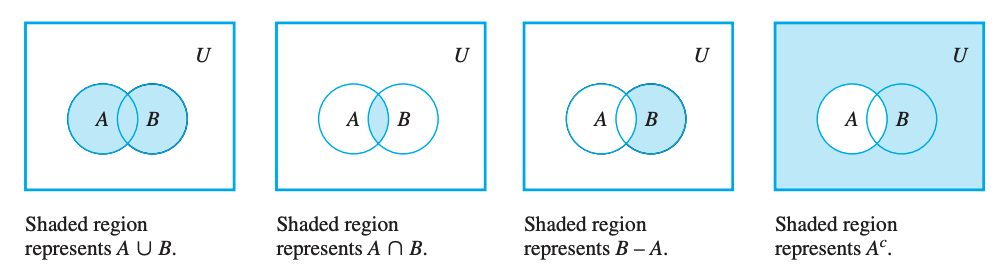
\includegraphics[scale=0.65]{setops}

\subsection{Disjoint Sets and Partitions}

A group of sets are \textbf{mutually disjoint} if the intersection of all pairs of sets is equal to
the empty set $\emptyset$.

\begin{definition}{Partition}{label}
    A finite or infinite collection of nonempty sets $\{A_1, A_2, A_3 \ldots\}$ is a \textbf{partition}
    of a set $A$ if, and only if,
    \begin{enumerate}
        \item $A$ is the union of all the $A_i$
        \item The sets $A_1,A_2,A_3 \ldots$ are mutually disjoint.
    \end{enumerate}
\end{definition}

\begin{definition}{Power Sets}{label}
    Given a set $A$, the \textbf{power set} of $A$, denoted $\wp(A)$, is the set of all subsets of $A$.
\end{definition}

\begin{definition}{Cartesian Product}{label}
    In general, \[
        A_1 \times A_2 \times \ldots A_n = \{(a_1, a_2, \ldots , a_n)  \mid a_1 \in A_1, a_2 \in A_2, \ldots , a_n \in A_n \}
    .\] 
    Note that $A_1 \times A_2 \times A_3$ is not quite the same thing as $(A_1 \times  A_2) \times A_3$
    because of tuple ordering.
\end{definition}

\section{Properties of Sets}

\begin{theorem}{Some Subset Relations}{label}
    \begin{enumerate}
        \item Inclusion of Intersection: $A \cap B \subseteq A$ and vice versa
        \item Inclusion in Union: $A \subseteq A \cup B$ and vice versa
        \item Transitive Property of Subsets: $A \subseteq B \land B \subseteq C \to A \subseteq C$
    \end{enumerate}
    To prove these theorems, \emph{suppose} that there is some arbitrary element of $A$ and show
    that it is also in $B$.
\end{theorem}

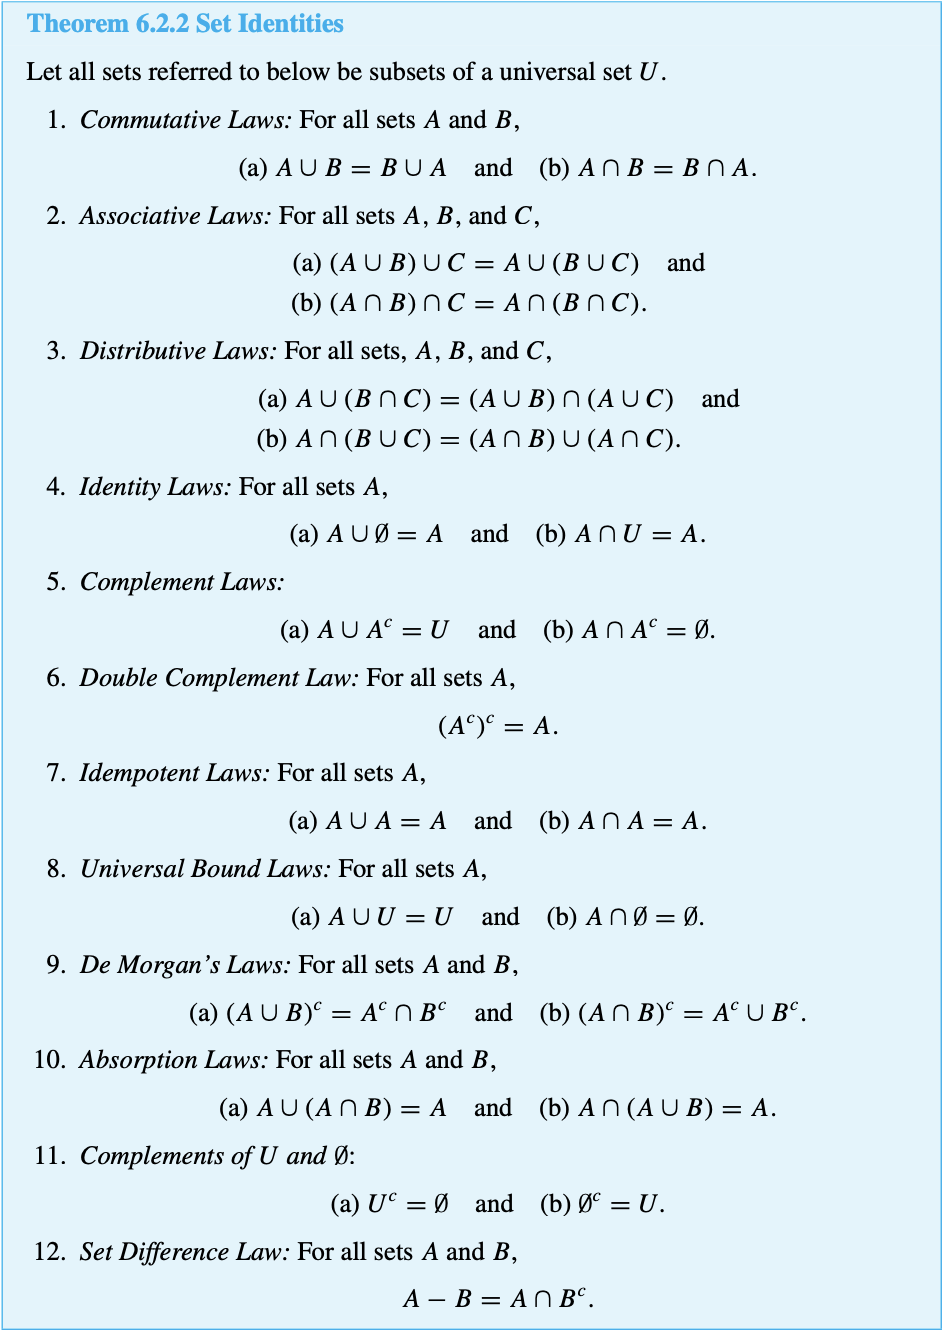
\includegraphics[scale=0.65]{setids}

In general, to prove set equality, you prove that set $A$ is a subset of set $B$, and that
set $B$ is a subset of set $A$. Additionally, to prove that a set $X$ is equal to the empty set
$\emptyset$, suppose $X$ has an element and derive a contradiction.

Additionally, casework is helpful when dealing with unions. It may be helpful to split a union into
2 cases.

\chapter{Functions}

In this chapter we go more in depth into properties of functions and their composition.

\section{Functions Defined on General Sets}

\begin{definition}{Function}{label}
    A \textbf{function} from a set $X$ to a set $Y$, denoted $f: X \to Y$, is a relation from
    $X$, the \textbf{domain}, to $Y$, the \textbf{co-domain}, that satisfies two properties:
    \begin{enumerate}
        \item Every element in $X$ is related to some element in $Y$
        \item No element in $X$ is related to more than one element in $Y$.
    \end{enumerate}
    The set of all values of $f$ is called the \emph{range of f} or the \emph{image of X under f}.
    If there exists some $x$ such that $f(x)=y$, then x is called a \textbf{preimage 
    (or inverse image) of $y$}.

    Two functions $F: X \to Y$ and $G: X \to Y$ are considered equal if, for all $x \in X, F(x) = G(x)$
\end{definition}

\begin{definition}{Identity Function}{label}
    The identity function $I_X$ is a function from $X \to X$ by which $I_X(x) = x \forall x \in X$.
\end{definition}

\begin{definition}{Logarithmic Function}{label}
    The log function $\log_b{x}=y$ (from $\mathbb{R}^{+}$ to $\mathbb{R}$) maps a number to the $y$ in the solution of
    the equation $b^y=x$.
\end{definition}

\subsection{Well Defined Functions}

We say that a function is \textbf{not well defined} if it fails to satisfy at least one of the
requirements for being a function. A function being well defined really means that it qualifies
to be called a function.

\section{One-to-One and Onto, Inverse Functions}

\subsection{One-to-one}

A function is \textbf{one-to-one} (or \textbf{injective}) if, and only if, every input has a unique 
output. Symbolically, $\forall x_1, x_2 \in X, f(x_1)=f(x_2) \to x_1 = x_2$.

To prove that $f$ is one-to-one, you \textbf{suppose} $x_1$ and $x_2$ are elements of $X$ such that
$f(x_1)=f(x_2)$, and \textbf{show} that $x_1=x_2$.

\subsection{Onto}

A function is \textbf{onto} (or \textbf{surjective}) if, and only if, the co-domain of the function
is equal to its image. Symbolically, $\forall y \in Y, \exists x \in X  \mid f(x) = y$.

To prove that $f$ is onto, you \textbf{suppose} $y$ is in $Y$, and \textbf{show} that
there exists an element in $x$ such that $y = f(x)$.

\subsection{One-to-one correspondences and Inverse Functions}

\begin{definition}{Bijection}{label}
    A \textbf{one-to-one correspondence} (or \textbf{bijection}) from a set $X$ to a set $Y$ is
    a function that is both one-to-one and onto.
\end{definition}

\begin{theorem}{Inverse Functions}{label}
    Suppose $F: X \to Y$ is a one-to-one correspondence. Then there is a function $F^{-1}: Y \to X$
    where $F^{-1}(y)=x$. Note that $F^{-1}$ is also a one-to-one correspondence.

    Additionally, note that \[
        f^{-1}(b) = a \Leftrightarrow f(a) = b
    .\] 
\end{theorem}

Finding an inverse function is done while proving that some function $F$ is onto.

\section{Composition of Functions}

The composition of functions (defined as $(g \circ f)(x) = g(f(x)) \forall x \in X$) for two
functions $f: X \to Y$ and $g: Y \to Z$ is $(g \circ f): X \to Z$.
Two compositions are equivalent if they have the same output for every input.

\begin{theorem}{Composition of a Function with Its Inverse}{label}
    $f^{-1} \circ f = I_X$ and $f \circ f^{-1} = I_Y$. This can be proved directly using the
\end{theorem}
\end{document}

